\documentclass[12pt, a4paper]{article}

\usepackage[utf8]{inputenc}
\usepackage[T1]{fontenc}
\usepackage[polish]{babel}
\usepackage{amsmath}
\usepackage{amssymb}
\usepackage{graphicx}
\usepackage{booktabs}
\usepackage{hyperref}
\usepackage{geometry}
\usepackage{caption}
\usepackage{float}

\geometry{margin=2.5cm}

\graphicspath{{./}}

\title{Podsumowanie prac}
\date{}

\begin{document}

\maketitle

% ---------------------------------------------------------------
\section{NARMA-30 --- test statystyczny}

 Zacząłem od eksperymentu, który porównuje tradycyjny ESN (ESNFeedback) z Isospectral ESN (ESNCustomizable) na zadaniu NARMA-30. Oba modele optymalizowane były przez 100 prób algorytmem Optuna, z rezerwuarem rozmiaru $N = 400$. Porównanie przeprowadzono w 10 niezależnych przebiegach. Zestawienie wyników zestawiono w Tabeli~\ref{tab:narma30}.

\begin{table}[H]
\centering
\begin{tabular}{lcc}
\toprule
Model & Średnie NMSE (test) & Odch. std \\
\midrule
ESNFeedback     & 0.3253 & 0.0643 \\
Isospectral ESN & \textbf{0.1719} & 0.0277 \\
\bottomrule
\end{tabular}
\caption{Wyniki na zadaniu NARMA-30. Metryka: NMSE uśrednione po 10 przebiegach.}
\label{tab:narma30}
\end{table}

Sparowany t-test wykazał istotną statystycznie różnicę na korzyść Isospectral ESN: $t = 6.56$, $p = 0.0001$ (przy $\alpha = 0.05$). Isospectral ESN uzyskuje NMSE o ok.\ 47\% niższe niż standardowy ESN. Jako, że NARMA-30 testuje głównie pamięć modelu, eksperyment pokazuje, że Isospectral ESN jest lepsza od tradycyjnych ESNów w tym zakresie. We wszystkich eksperymentach optymalny rozkład warotści własnych był blisko krawędzi jednostkowego dysku.

\begin{figure}[H]
    \centering
    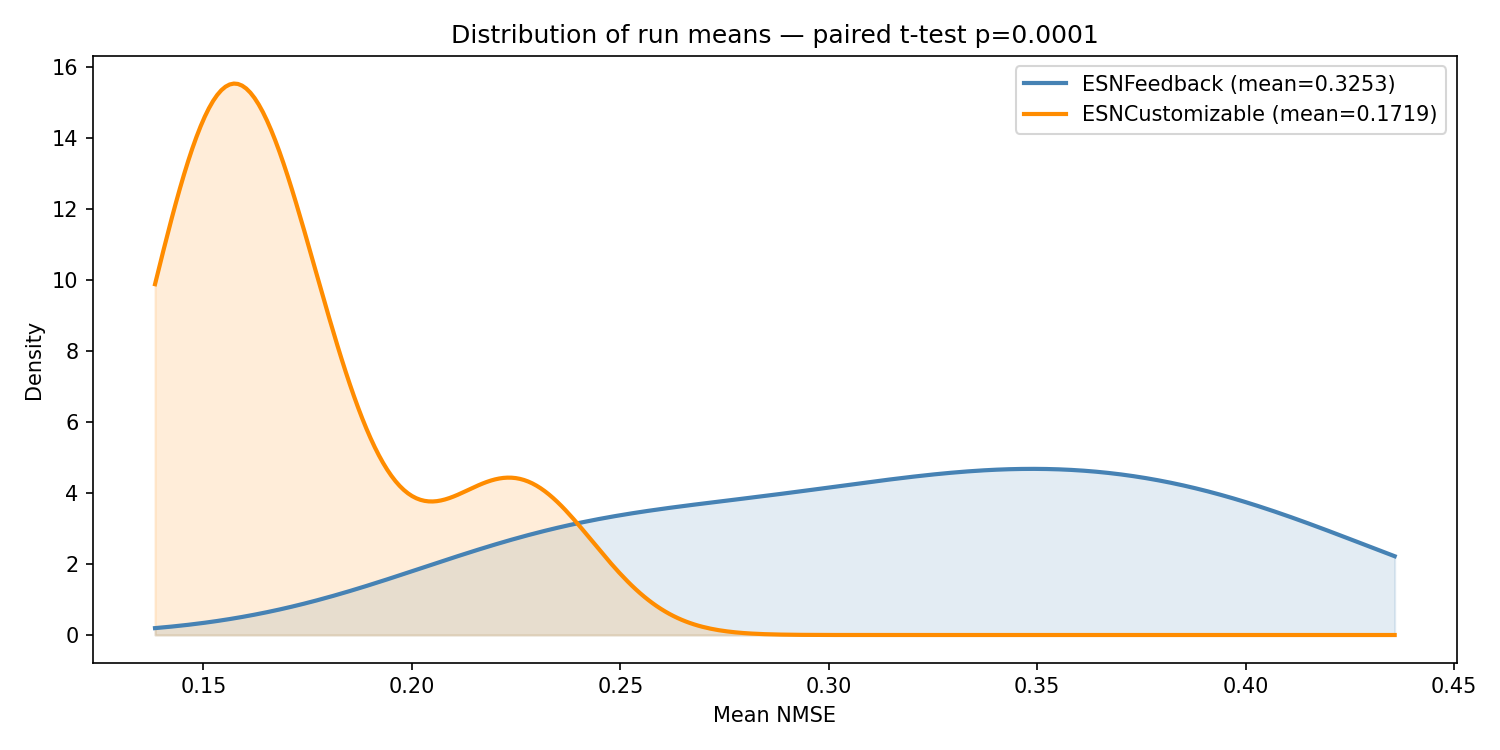
\includegraphics[width=0.85\textwidth]{experiments/experiment_53/test_score_distribution.png}
    \caption{Rozkład NMSE na zbiorze testowym po wszystkich przebiegach, NARMA-30.}
\end{figure}

\begin{figure}[H]
    \centering
    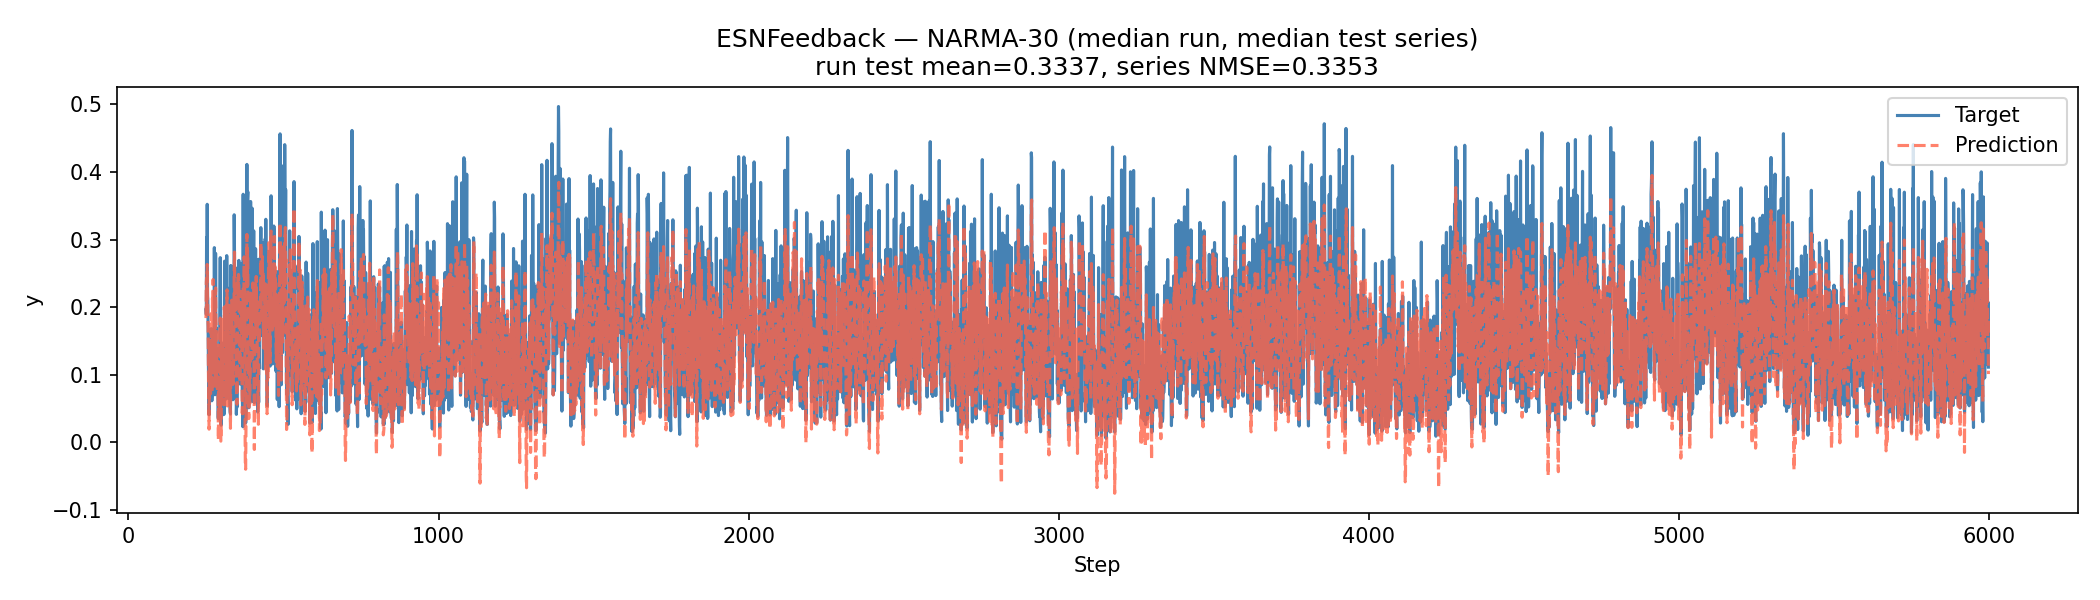
\includegraphics[width=\textwidth]{experiments/experiment_53/predictions_a.png}
    \caption{Predykcje ESNFeedback na zbiorze testowym, NARMA-30.}
\end{figure}

\begin{figure}[H]
    \centering
    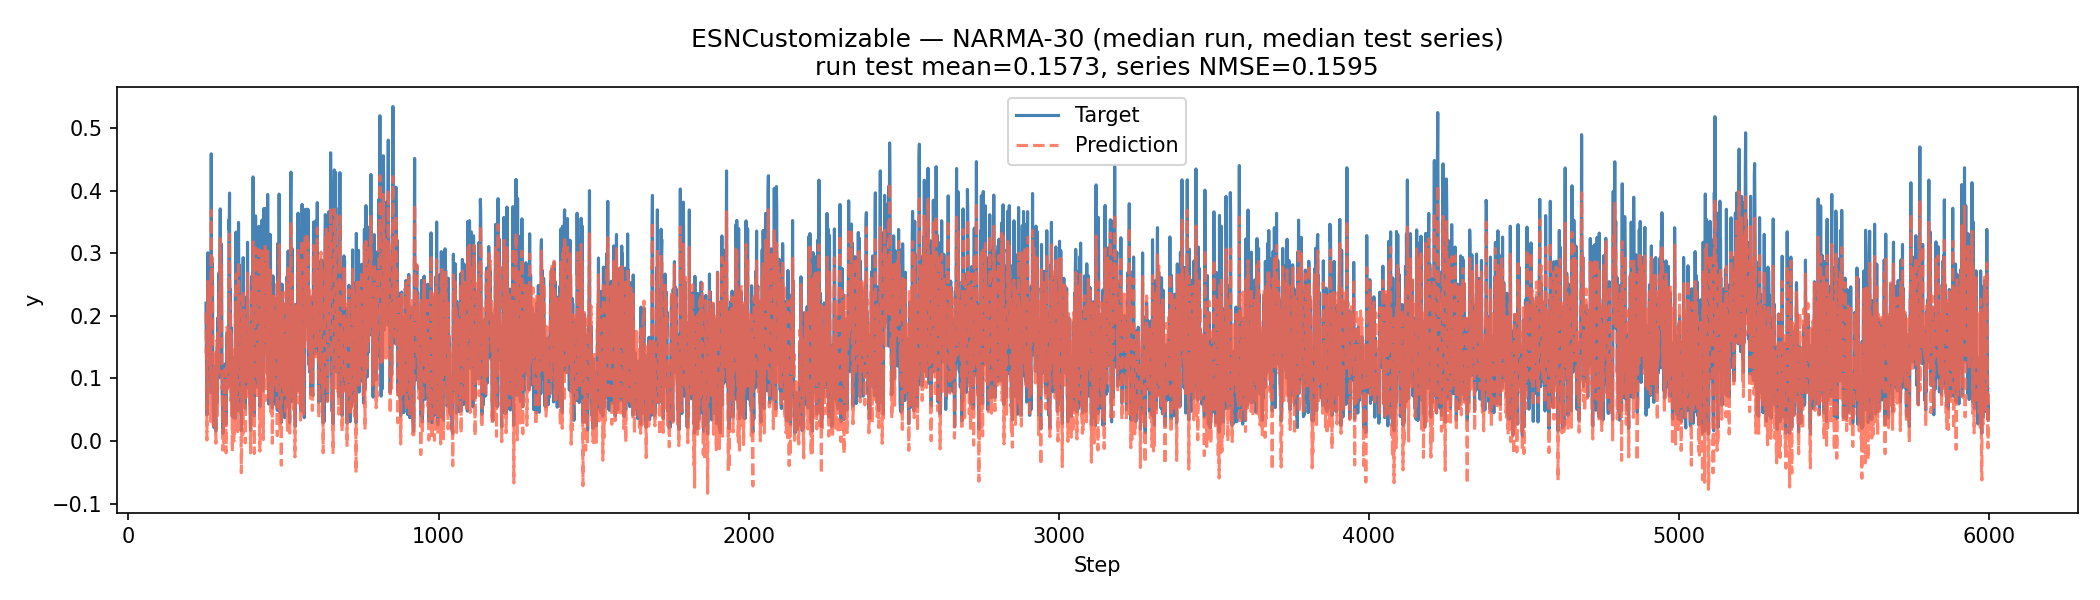
\includegraphics[width=\textwidth]{experiments/experiment_53/predictions_b.png}
    \caption{Predykcje Isospectral ESN na zbiorze testowym, NARMA-30.}
\end{figure}

% ---------------------------------------------------------------
\section{Mackey-Glass i Lorenz}

Zadania predykcji autonomicznej (Mackey-Glass i Lorenz) różnią się od NARMA tym, że nie ma zewnętrznego wejścia --- model po fazie rozgrzewania generuje trajektorię, podając własne wyjście jako wejście do kolejnego kroku. Metryka to liczba kroków do dywergencji predykcji od rzeczywistej trajektorii.

\subsection{Mackey-Glass}

Eksperyment 44 porównuje oba modele na 20 niezależnych przebiegach (różne ziarna optymalizatora). Wyniki zestawiono w Tabeli~\ref{tab:mg}.

\begin{table}[H]
\centering
\begin{tabular}{lcc}
\toprule
Model & Średnia liczba kroków (test) & Odch. std \\
\midrule
ESNFeedback     & 396.7 & 86.1 \\
Isospectral ESN & 402.7 & 74.3 \\
\bottomrule
\end{tabular}
\caption{Wyniki na zadaniu Mackey-Glass. Metryka: liczba kroków do dywergencji.}
\label{tab:mg}
\end{table}

Sparowany t-test nie wykazał istotnej różnicy: $t = -0.24$, $p = 0.81$. Oba modele uczą dynamiki układu do pewnego horyzontu, po którym trajektoria  dywerguje ze względu na chaotyczny charakter systemu. Test Wilcoxona potwierdza ten wynik: $W = 516.5$, $p = 0.24$ (nieistotne).

\begin{figure}[H]
    \centering
    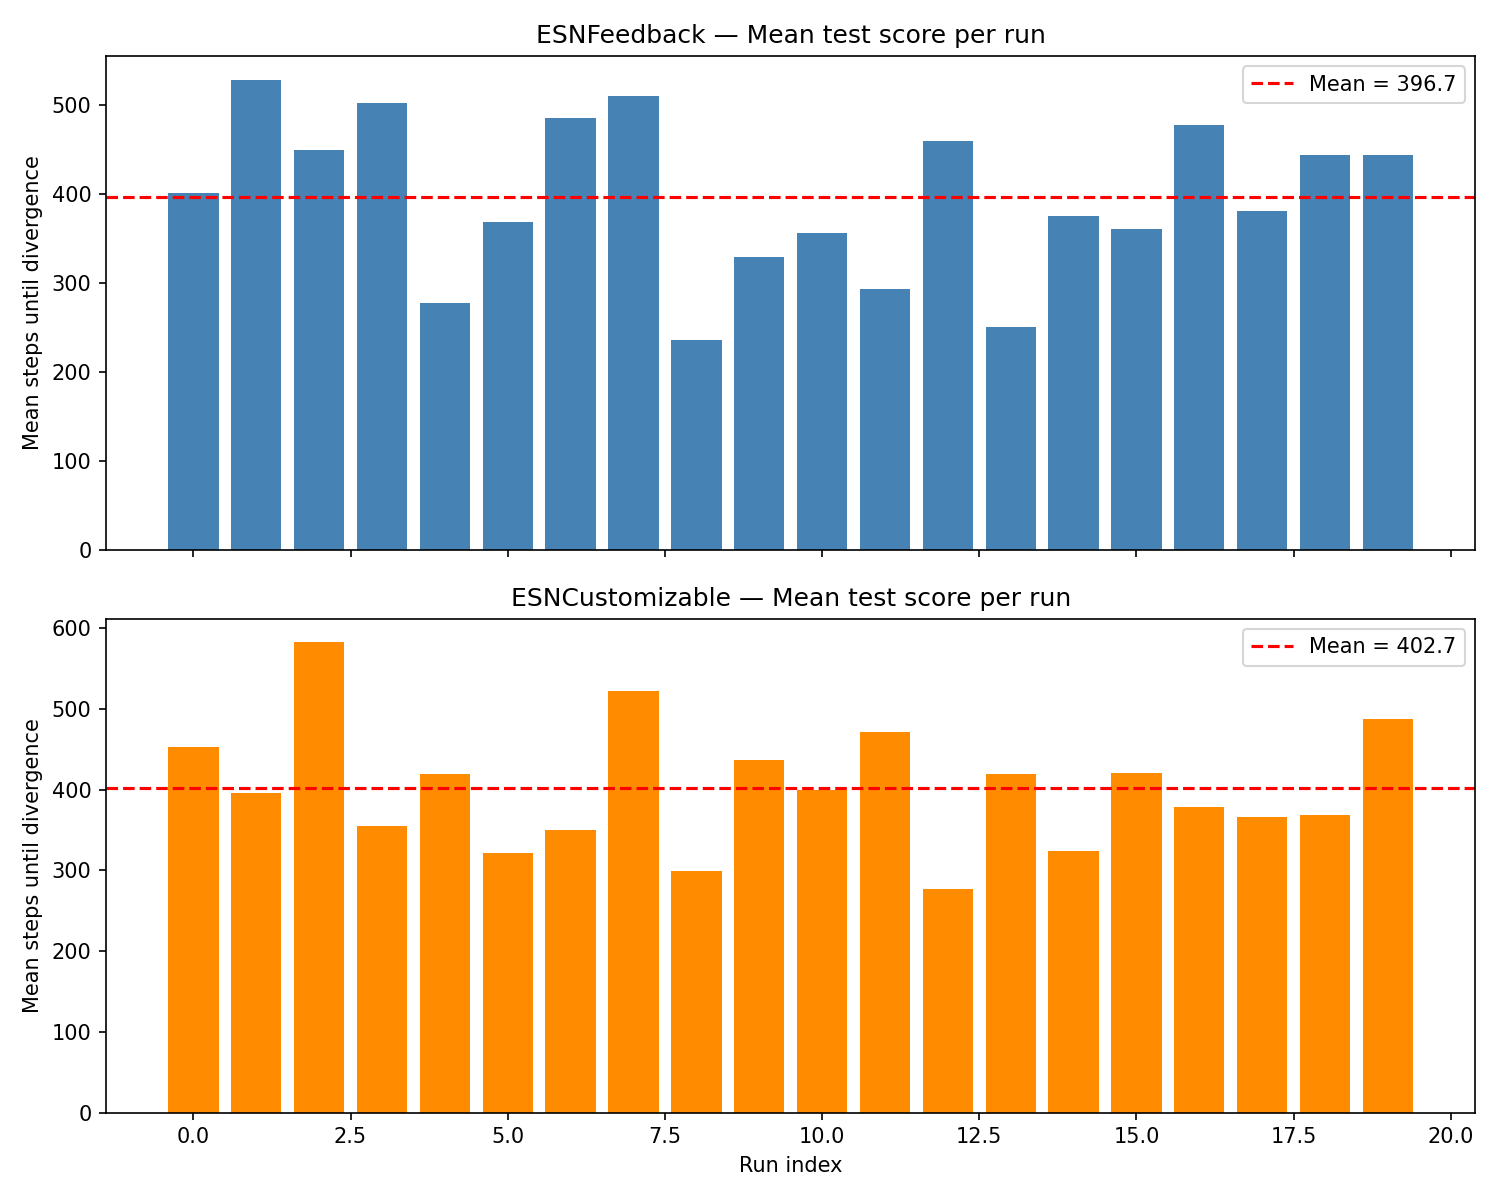
\includegraphics[width=0.85\textwidth]{experiments/experiment_44/test_steps_bar.png}
    \caption{Liczba kroków do dywergencji dla każdego przebiegu, Mackey-Glass.}
\end{figure}

\begin{figure}[H]
    \centering
    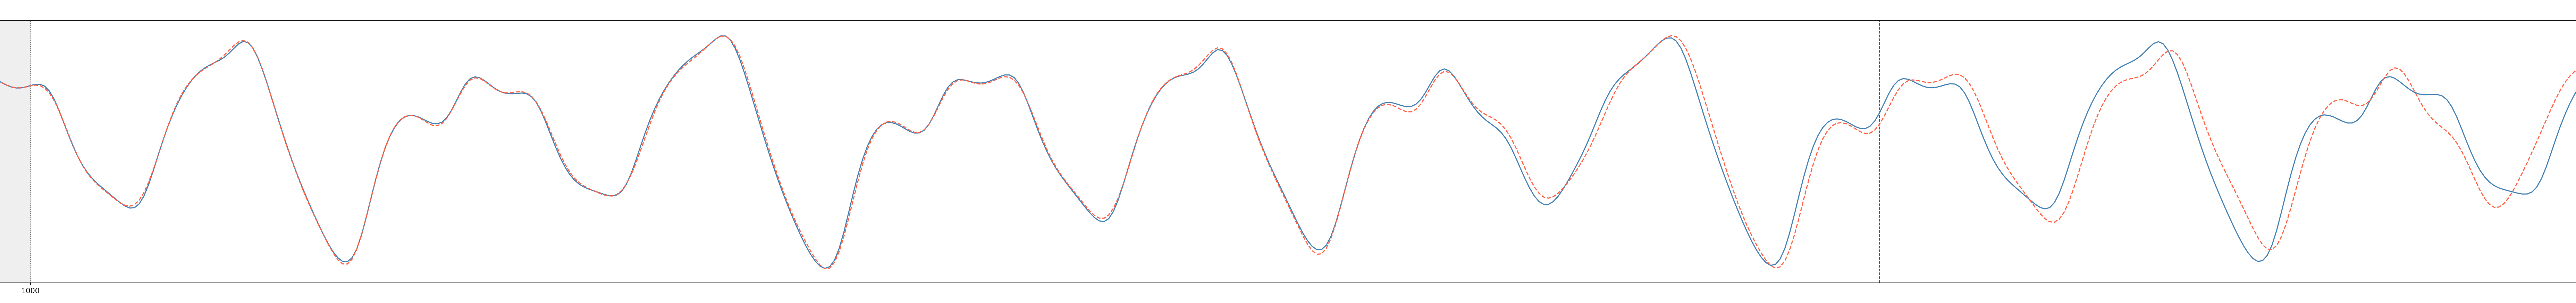
\includegraphics[width=\textwidth]{img/exp43_predictions_a.png}
    \caption{Predykcja autonomiczna ESNFeedback, Mackey-Glass. Pomarańczowa przecinana linia pokazuje punkt dywergencji.}
\end{figure}

\begin{figure}[H]
    \centering
    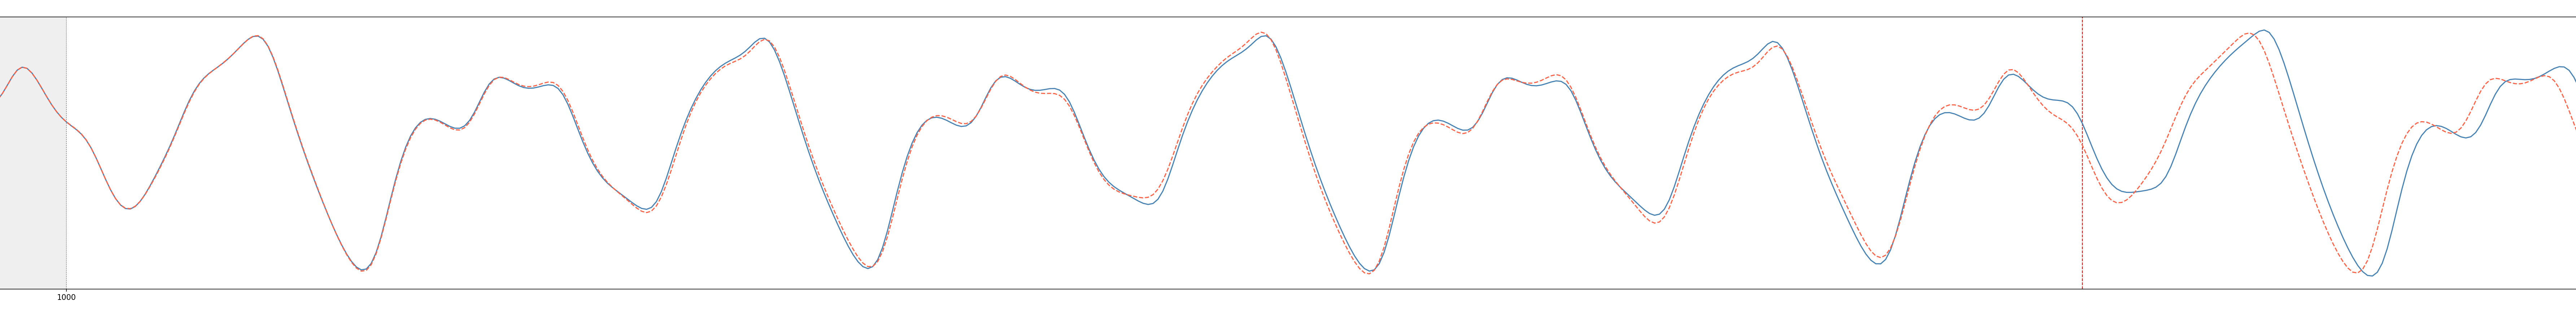
\includegraphics[width=\textwidth]{img/exp43_predictions_b.png}
    \caption{Predykcja autonomiczna Isospectral ESN, Mackey-Glass. Pomarańczowa przecinana linia pokazuje punkt dywergencji.}
\end{figure}

\subsection{Lorenz}

Układ Lorenza jest trudniejszym benchmarkiem niż Mackey-Glass z uwagi na silniejszy chaos. Eksperymenty testują odpowiednio ESNFeedback i Isospectral ESN (osobno, na razie brak testów statystycznych). Wyniki zestawiono w Tabeli~\ref{tab:lorenz}.

\begin{table}[H]
\centering
\begin{tabular}{lcc}
\toprule
Model & Średnia liczba kroków (test) & Odch. std \\
\midrule
ESNFeedback     & 69.9 & 32.1 \\
Isospectral ESN & 50.0 & 21.4 \\
\bottomrule
\end{tabular}
\caption{Wyniki na zadaniu Lorenz.}
\label{tab:lorenz}
\end{table}

Wyniki obu modeli mieszczą się w podobnym przedziale, przy dużej wariancji między inicjalizacjami. Wyniki sugerują brak dominacji któregokolwiek z modeli.

\begin{figure}[H]
    \centering
    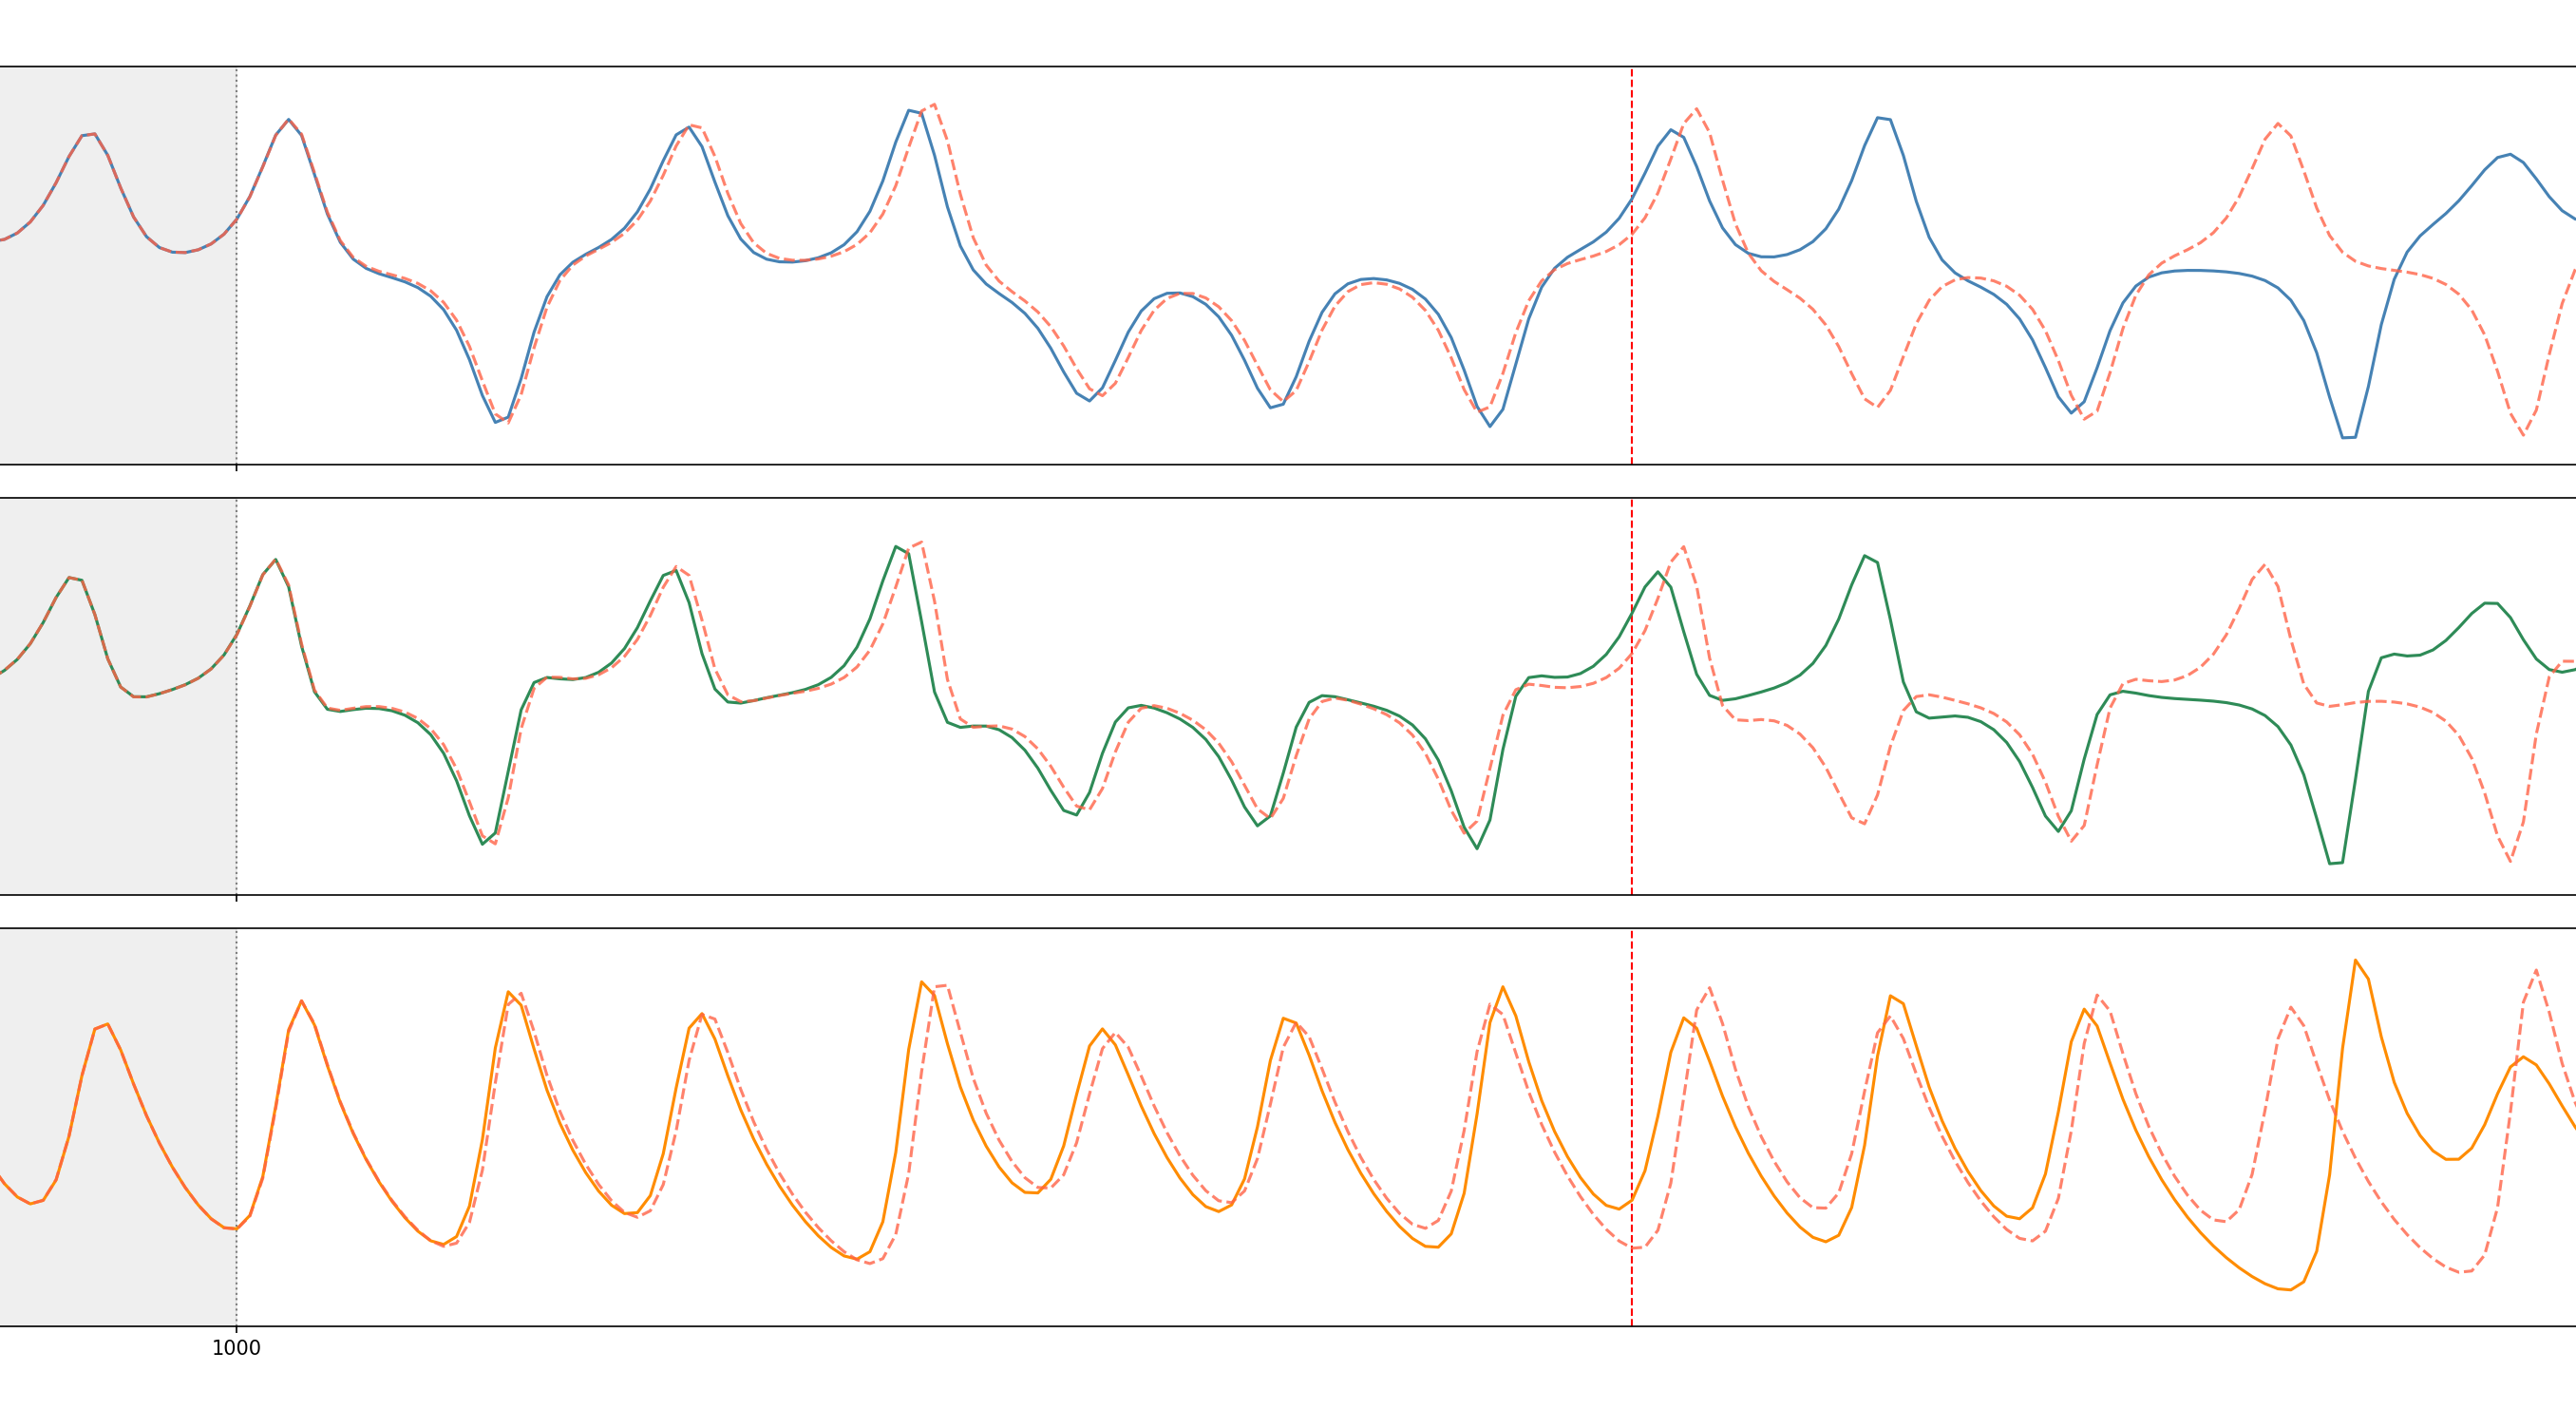
\includegraphics[width=\textwidth]{img/exp41_predictions.png}
    \caption{Predykcja autonomiczna ESNFeedback, układ Lorenza. Pomarańczowa przecinana linia pokazuje punkt dywergencji.}
\end{figure}

\begin{figure}[H]
    \centering
    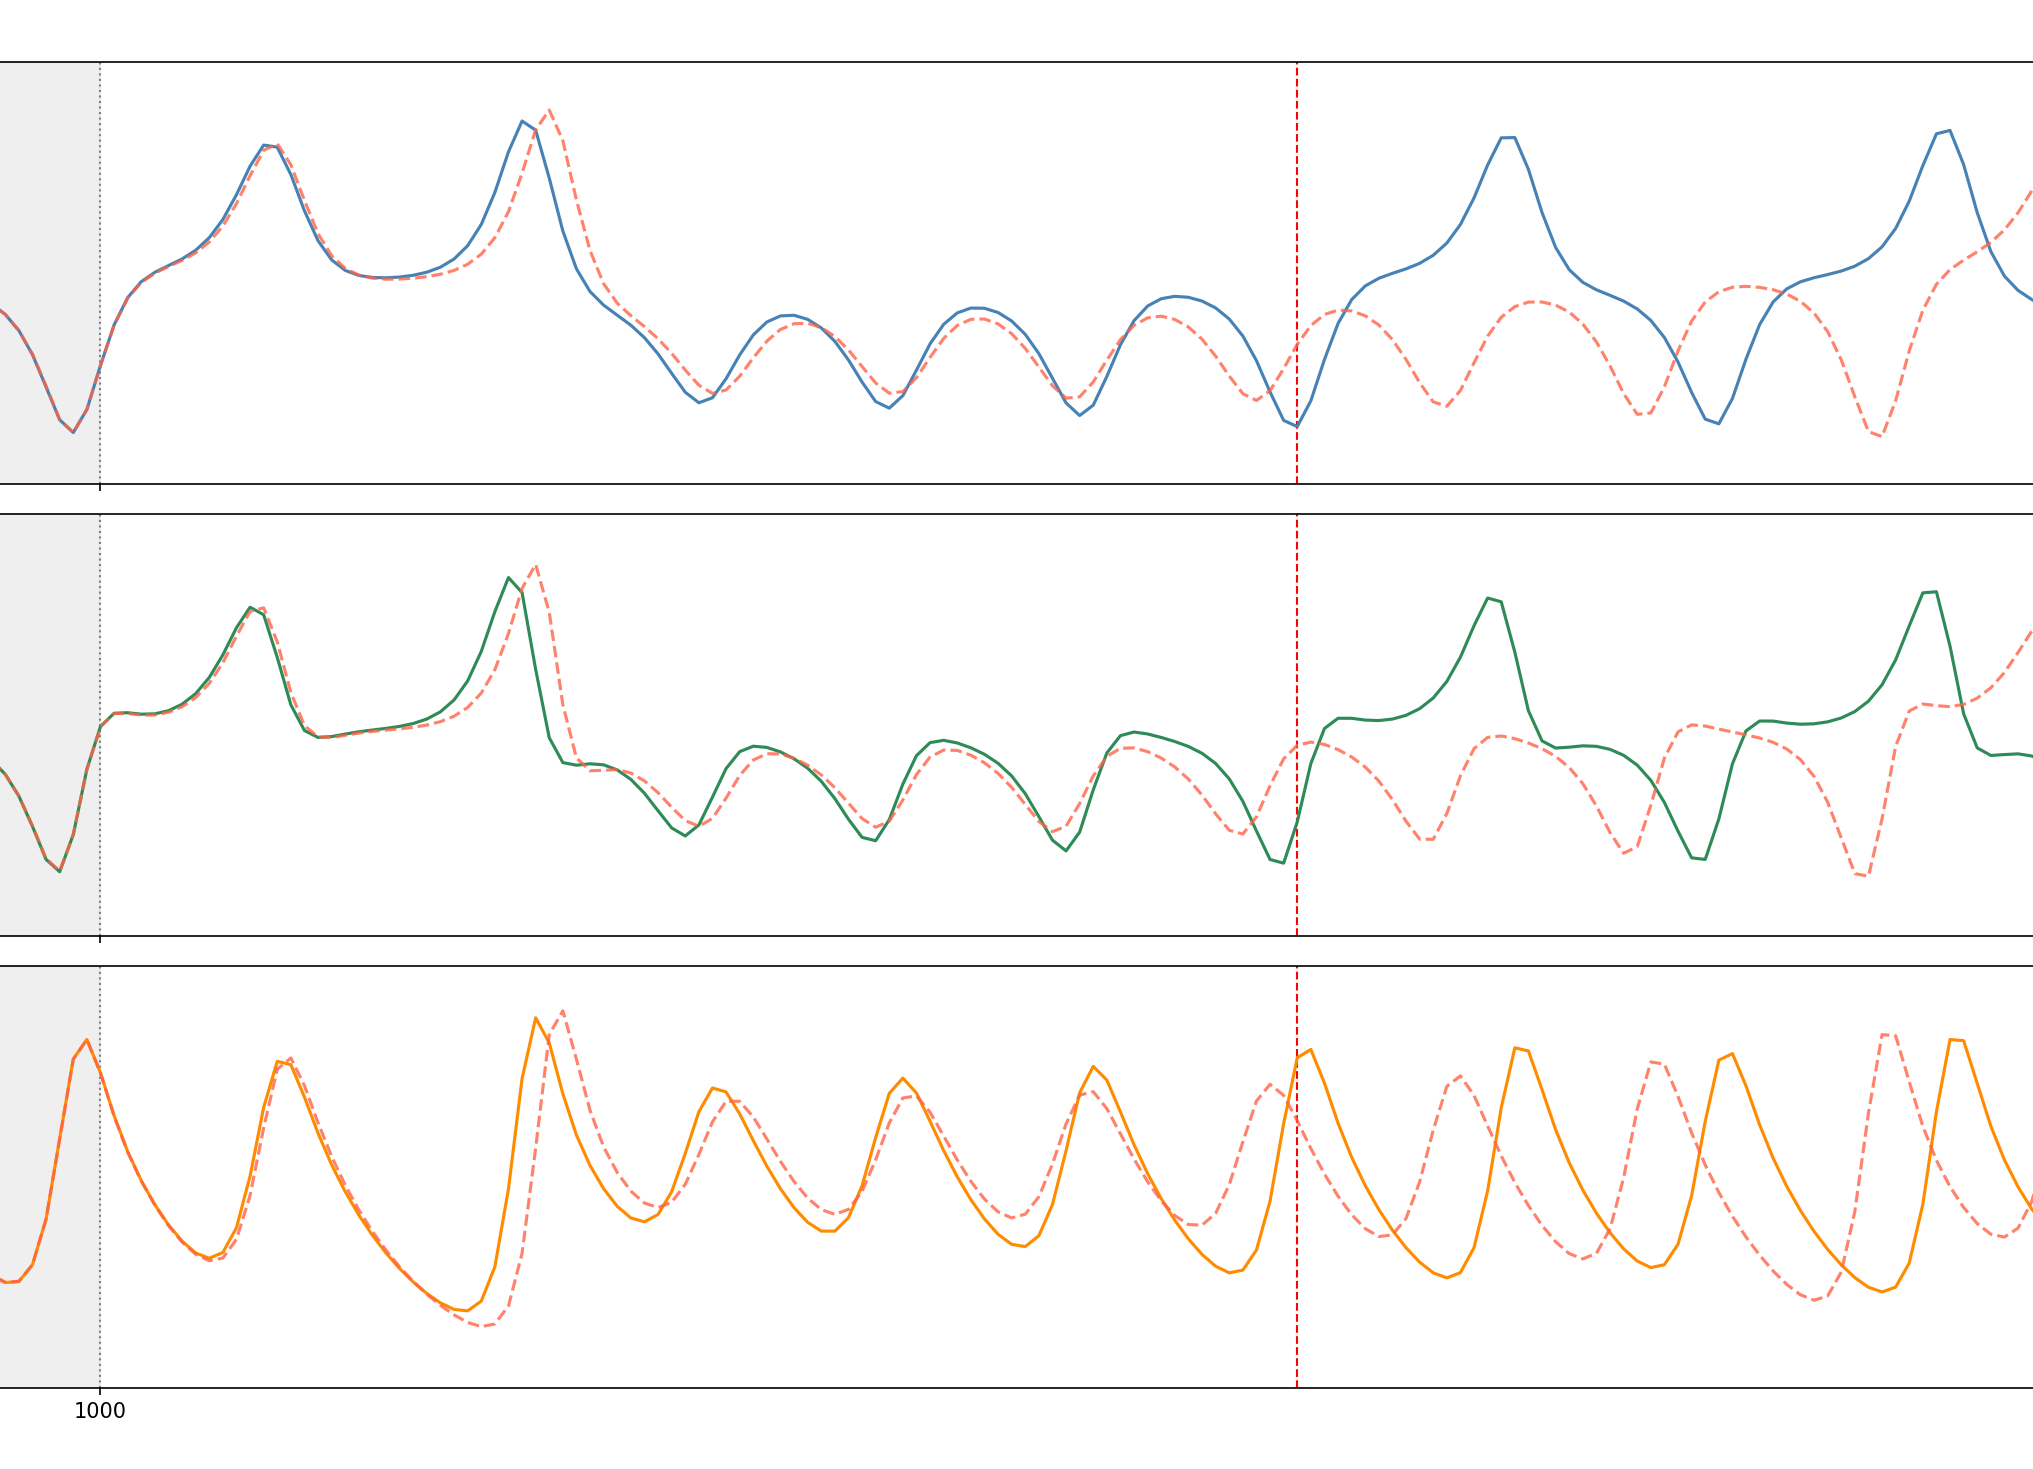
\includegraphics[width=\textwidth]{img/exp47_predictions.png}
    \caption{Predykcja autonomiczna Isospectral ESN, układ Lorenza. Pomarańczowa przecinana linia pokazuje punkt dywergencji.}
\end{figure}

\subsection{Komentarz}

Wyniki na obu zadaniach chaotycznych wskazują, że Isospectral ESN nie uzyskuje przewagi nad standardowym ESN. Kontrola rozkładu wartości własnych, która skutkuje istotną poprawą na NARMA-30 (zadanie z pamięcią), nie przekłada się na lepszą predykcję chaotycznych układów dynamicznych. Możliwym wyjaśnieniem jest to, że kluczowym czynnikiem w tych zadaniach jest właściwa stabilność numeryczna podczas autonomicznej inferencji, a niekoniecznie pamięć. 

% ---------------------------------------------------------------
\section{Dalsze prace}

Aktualnie planuję  eksperymenty z rzeczywistymi zbiorami danych. Celem jest sprawdzenie, czy model nadaje się do predykcji szeregów czasowych spoza syntetycznych benchmarków. Planuję sprawdzić kilka datasetów:

\begin{itemize}
    \item \textbf{Prognozowanie zużycia energii elektrycznej} --- zbiór \textit{ElectricityLoadDiagrams} zawierający pomiary obciążenia 370 klientów w interwałach 15-minutowych. Zadanie polega na krótkoterminowej prognozie zużycia.
    \item \textbf{Cymatyka} --- -
    \item \textbf{Prognozowanie wiatru} --- rzeczywiste dane meteorologiczne
\end{itemize}

Poza tym spróbuję jeszcze polepszyć działanie modelu na zadaniach Lorenz i Mackey-Glass.

\end{document}
